\documentclass{beamer}


\title{Reinforcement Learning}
\author{
    Niccolò Consigli
		\scriptsize \texttt{n.consigli@studenti.unipi.it}
		\\
		\normalsize
    Luca Seggiani
		\scriptsize \texttt{l.seggiani@studenti.unipi.it}
		\normalsize
	}
\institute{Università di Pisa}
\date{\today}

\begin{document}

\begin{frame}
	\titlepage
\end{frame}

\begin{frame}
	\frametitle{A new kind of learning}
	\begin{itemize}
		\item<1-> Supervised learning: matching features to labels
		\item<2-> Unsupervised learning: clustering data
		\item<3-> \textbf{Reinforcement learning}: learning from rewards
	\end{itemize}
\end{frame}

\begin{frame}
	\frametitle{What is reinforcement learning (RL)?}
	\begin{itemize}
		\item<1-> We give the agent \textbf{rewards} based on its performance
		\item<2-> Markov property: we can view problems as \textbf{Markov decision processes} (MDPs)
	\end{itemize}
\end{frame}

\begin{frame}
	\frametitle{A framework: Markov decision processes}
	\begin{itemize}
		\item Actions map states to states with a probability distribution
		\item Transition reward: $R(s, a, s')$
		\item Transition probability: $P(s' \, | \, s, a)$
	\end{itemize}
	\begin{center}
		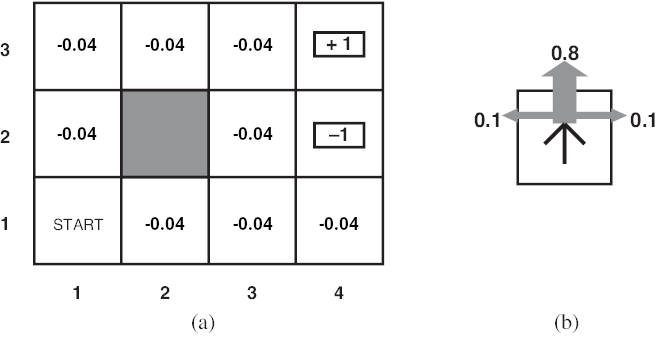
\includegraphics[scale=0.95]{figures/markov-decisional-process.png}
	\end{center}
	\pause
	\begin{block}{Bellman's equation}
		Given a discount factor $\gamma \in [0, 1]$, the utility is given by:
		$$
		U(s) = \max_{a \in A(s)} \sum_{s'} P(s' \, | \, s, a) \left[ R(s, a, s') + \gamma U(s') \right]
		$$
	\end{block}
\end{frame}

\begin{frame}
	\frametitle{Model-based reinforcement learning}
	We maintain a transition model (an \textbf{MDP}):
	\begin{itemize}
		\item Reward function: $R(s, a, s')$
		\item Probability function: $P(s' \, | \, s, a)$
		\item Utility function: U(s), maps states to \textbf{utility}
	\end{itemize}
	\pause
	Once the model is learned, we can \textbf{maximize utility}
	\begin{center}
		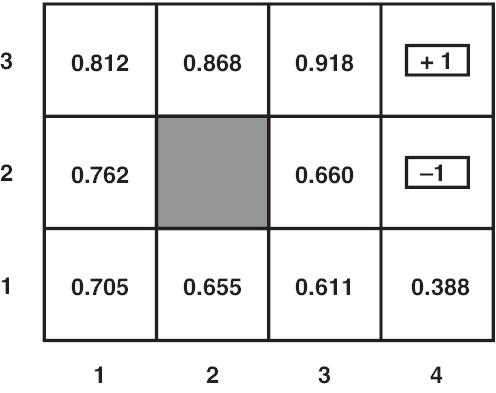
\includegraphics[scale=0.8]{figures/optimal-policy-values.png}
	\end{center}
\end{frame}

\begin{frame}
	\frametitle{Model-free reinforcement learning}
	\begin{itemize}
		\item Action-utility function: $Q(s, a)$ maps \textbf{actions} to \textbf{utility}
		\item Policy search: maps \textbf{states} to \textbf{actions}, essentialy a reflex agent
	\end{itemize}
	\begin{center}
		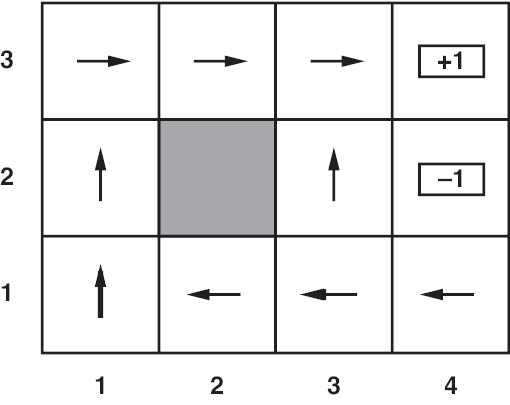
\includegraphics[scale=0.8]{figures/optimal-policy-arrows.png}
	\end{center}
\end{frame}

\begin{frame}
	\frametitle{Passive reinforcement learning}
	We can't modify the policy, but we can figure out the utilities $U(s)$
	\begin{itemize}
		\item We use \textbf{policy iteration}:
			$$
				U^\pi(s) = E\left[ \sum_{t=0}^{+\infty} \gamma^t R(s_t, \pi(s_t), s_{t+1}) \right]
			$$
	\end{itemize}
	\pause
	Three approaches for approximation:
	\begin{itemize}
		\item Direct estimation
		\item Adaptive dynamic programming (ADP)
		\item Temporal difference learning (TD)
	\end{itemize}
\end{frame}

\begin{frame}
	\frametitle{Direct estimation}
	The goal is to approximate state utility under the given policy
	\begin{itemize}
		\item Make \textbf{trials} and take the \textbf{reward-to-go} for each state
	\end{itemize}
	\pause
	\begin{block}{Example}
	We calculate utilities for $(1,2)$ given the trial:
		$$
		\scriptstyle
		(1,1) \xrightarrow[\mathrm{Up}]{-0.4} 
		(1,2) \xrightarrow[\mathrm{Up}]{-0.4}
		(1,3) \xrightarrow[\mathrm{Right}]{-0.4}
		(1,2) \xrightarrow[\mathrm{Up}]{-0.4}
		(1,3) \xrightarrow[\mathrm{Right}]{-0.4}
		(2,3) \xrightarrow[\mathrm{Right}]{-0.4}
		(3,3) \xrightarrow[\mathrm{Right}]{+1}
		(4,3)
	$$
	\pause
	$$
		U(1,2) = -0.04 -0.04 -0.04 -0.04 -0.04 + 1 = 0.8
	$$
	\pause
	$$
		U(1,2)' = -0.04 -0.04 -0.04 + 1 = 0.88
	$$
	\end{block}
	\pause
	\begin{itemize}
		\item This is inefficient! We can \textbf{exploit} the Markov property 
	\end{itemize}
\end{frame}

\begin{frame}
	\frametitle{Adaptive dynamic programming}
	We can approximate the transition reward and probability functions ($P$ and $R$) and apply \textbf{simplified Bellman's equation}:
	$$
		U(s) = \sum_{s'} P(s' \, | \, s, \pi(s)) \left[ R(s, \pi(s), s') + \gamma U(s') \right]
	$$
	When the policy is fixed, this gives a \textbf{linear equation}
	\pause
	\begin{itemize}
		\item Calculating $P$ and $R$ is easy when the environment is \textbf{fully observable} 
	\end{itemize}
\end{frame}

\begin{frame}
	\frametitle{Temporal difference learning}
	Still taking trials, but we \textbf{update} the utility to match frequently observed transitions
	\pause
	\begin{block}{Example}
	We calculate utilities for $(1,3)$ given the trial:
		$$
		\scriptstyle
		(1,1) \xrightarrow[\mathrm{Up}]{-0.4} 
	(1,2) \xrightarrow[\mathrm{Up}]{-0.4}
	(1,3) \xrightarrow[\mathrm{Right}]{-0.4}
	(2,3) \xrightarrow[\mathrm{Right}]{-0.4}
	(3,3) \xrightarrow[\mathrm{Right}]{-0.04}
	(3,2) \xrightarrow[\mathrm{Up}]{-0.04}
	(3,3) \xrightarrow[\mathrm{Right}]{+1}
	(4,3)	
	$$
	\pause
	$$
		U^\pi (1, 3) = -0.04 + U^\pi (2,3)
	$$
	\end{block}
	\pause
	Then we can update with learning rate $\alpha$:
	$$
	U^\pi(s) \leftarrow U^\pi(s) + \alpha \left[ R(s, \pi(s), s') + \gamma U^\pi (s') - U^\pi (s) \right]
	$$
	\begin{itemize}
		\item From TD's point of view, ADP is TD with \textit{simulated experiences}
	\end{itemize}
\end{frame}

\end{document}
